\documentclass{beamer}
\usetheme{CambridgeUS}
\usepackage[french]{babel}
\usepackage[T1]{fontenc}
\usepackage{hyperref}
\usepackage{tkz-graph}
\usepackage[linesnumbered,ruled,french,onelanguage]{algorithm2e}

\title{- Soutenance de projet -  }
\subtitle{Solveur de Ricochet Robots}
\author{ANDRÉ Lorada  \\ AUVRAY Théo}
\institute{L2 Informatique \\ Groupe 1A}
\date{\today}

% Pour algorithm2me---------------------------------------------
\SetKwRepeat{Do}{do}{while}%
\makeatletter 
\g@addto@macro{\@algocf@init}{\SetKwInput{KwOut}{Sortie}}
\makeatother


\begin{document}
%---------------------------------------------------------------
\begin{frame}
	\begin{figure}
        
\includegraphics[scale=0.5]{images/logo.png}
	\end{figure}
	\titlepage
\end{frame}
%---------------------------------------------------------------
\section{Sommaire}
    \begin{frame}{Sommaire}
        \tableofcontents
    \end{frame}
%---------------------------------------------------------------
\section{Introduction}
    \begin{frame}{Introduction}
        \begin{itemize}
            \item Le Ricochet Robots: jeu de société composé d'un plateau, de pions de robots et de jetons. 
            \vspace{0.25cm}
            \item Principe: Déplacer les robots pour atteindre la case qui correspond au symbole du jeton ayant été tiré aléatoirement. Le déplacement des robots s'effectue qu'en ligne droite jusqu'à rencontrer un obstacle (un robot ou un mur).
            
            \vspace{0.25cm}
            
            \item Objectifs: 
            \begin{itemize}
                \item Conception du Ricochet Robots.
                \item Réalisation d'une interface graphique.
                \item Implantation de l'algorithme A*, optimisation de l'algorithme.
            \end{itemize}
        \end{itemize}
    \end{frame}
%---------------------------------------------------------------
\section{Organisation}
    \begin{frame}{Organisation du projet}
        \begin{figure}
            \centering
            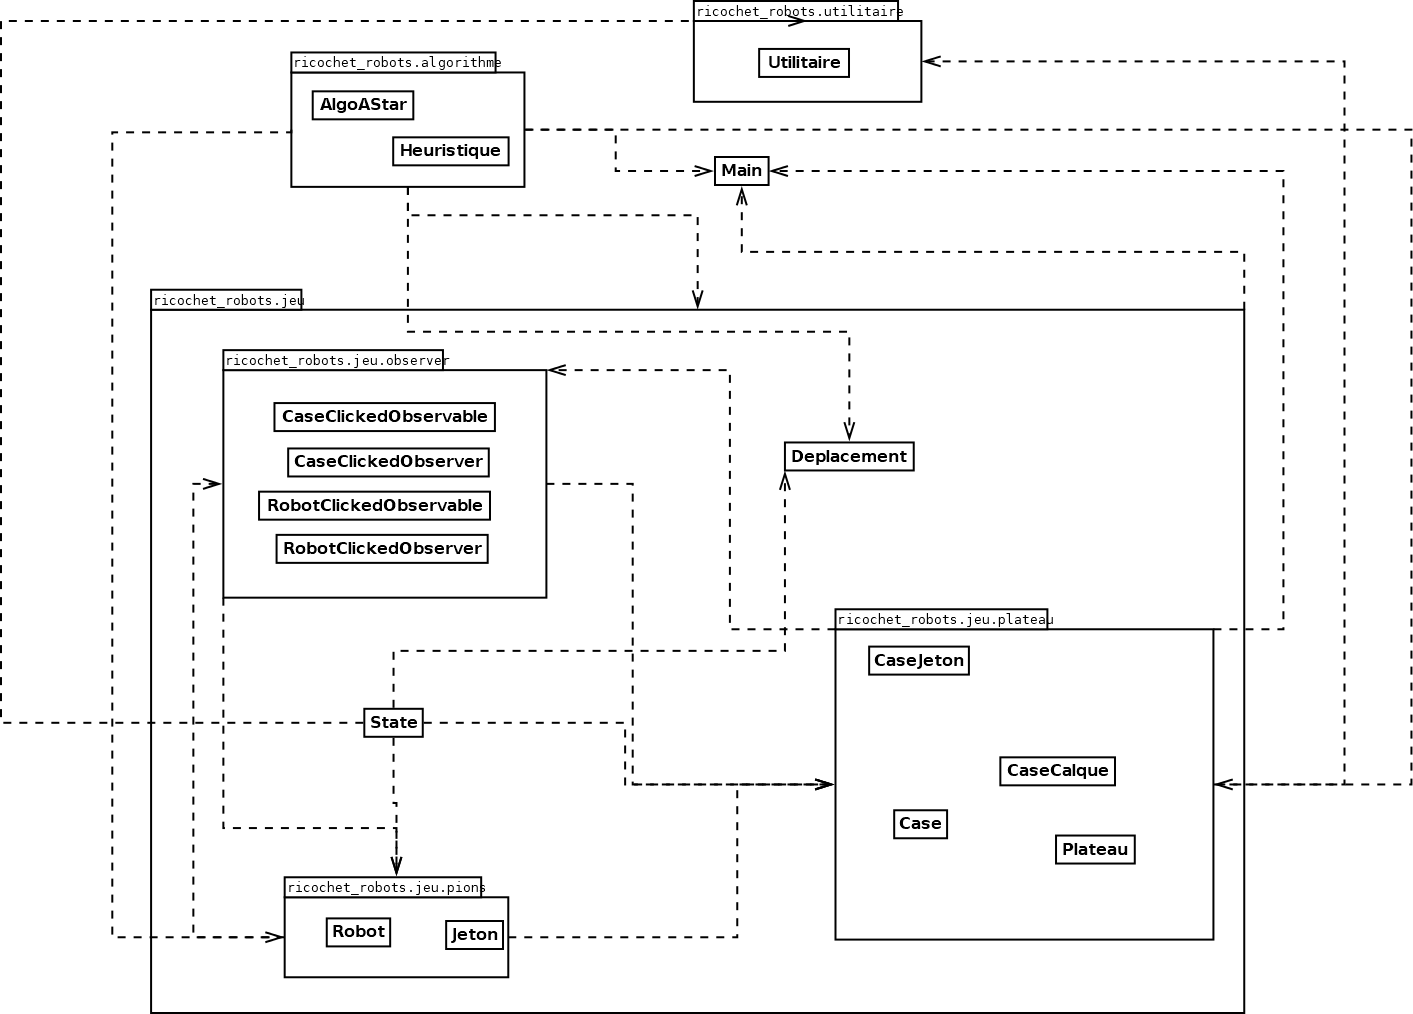
\includegraphics[scale=0.2]{images/DiagrammePackage.png}
        \end{figure}
    \end{frame}
%---------------------------------------------------------------
\section{Éléments techniques}
    \subsection{Création du plateau}
        \begin{frame}{Composition du plateau}
            \begin{columns}
                \begin{column}{6cm}
                    \begin{figure}
                        \centering
                        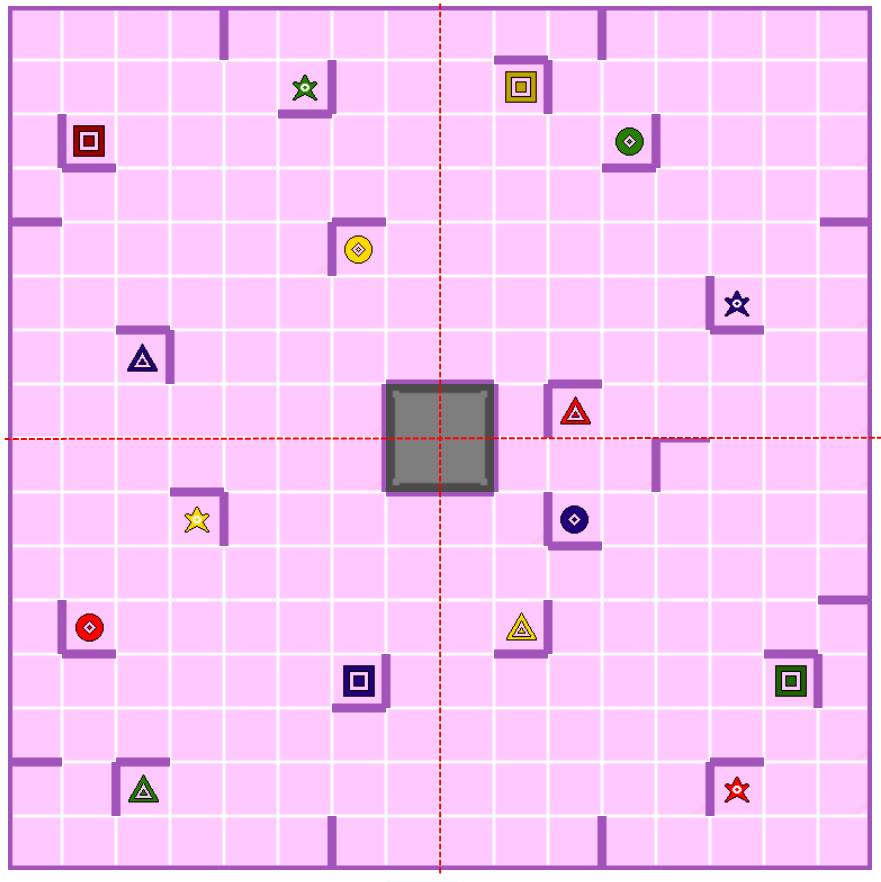
\includegraphics[scale=0.2]{images/plateau.png}
                    \end{figure}
                \end{column}
                \begin{column}{6cm}
                    \begin{figure}
                        \centering
                        
\includegraphics[scale=0.4]{images/listeRobots.png}
                        \caption{Liste des différents robots}
                    \end{figure}
                    \begin{figure}
                        \centering
                        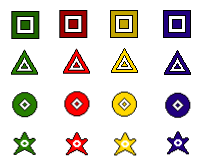
\includegraphics[scale=0.3]{images/listeJeton.png}
                        \caption{Liste des différents jetons}
                    \end{figure}
                    \begin{figure}
                        \centering
                        
\includegraphics[scale=0.2]{images/liste_cases.png}
                        \caption{Liste des différentes cases}
                    \end{figure}
                \end{column}
            \end{columns}
        \end{frame}
%---------------------------------------------------------------
            \begin{frame}{Composition des cases}
    
                \begin{tikzpicture}[]
                    \draw (1,1) rectangle (3,3);
                    \draw[color=red] (1,1.25) -- (3,1.25);
                    \draw[color=green] (1,2.75) -- (3,2.75);
                    \draw[color=blue] (1.25,1) -- (1.25,3);
                    \draw[color=olive] (2.75,3) -- (2.75,1);
                    \node[color=red] (pos) at (2,0.5) {BAS};
                    \node[color=green] (pos) at (2,3.5) {HAUT};
                    \node[color=blue] (pos) at (0,2) {DROIT};
                    \node[color=olive] (pos) at (4,2) {GAUCHE};
                    
                    \node (posi) at (8,2) {[ HAUT, DROIT, BAS, GAUCHE ]};
                \end{tikzpicture}
                \begin{center}
                    \begin{tikzpicture}
                        \draw[fill=red] (0,2) rectangle (2, 1.75);
                        \draw (0,0) rectangle (2,2);
                        \draw[dotted] (0,0.25) -- (2,0.25);
                        \draw[dotted] (0,1.75) -- (2,1.75);
                        \draw[dotted] (0.25,0) -- (0.25,2);
                        \draw[dotted] (1.75,0) -- (1.75,2);
                        
                        \node (bool) at (6,1) {[ True, False, False, False ]};
                        \node (bin) at (10,1) {[1,0,0,0]};
                        \draw[->] (bool) -- (bin);
                        \draw[->] (2.5,1) -- (bool);
                    \end{tikzpicture}
                \end{center}
                
            \end{frame}
%---------------------------------------------------------------
            \begin{frame}{Positionnement des mini-plateaux}
                \begin{columns}
                    \begin{column}{6cm}
                        
                         On affecte par exemple à ce plateau la position 3.
                         
                        \begin{figure}
                            \centering
                            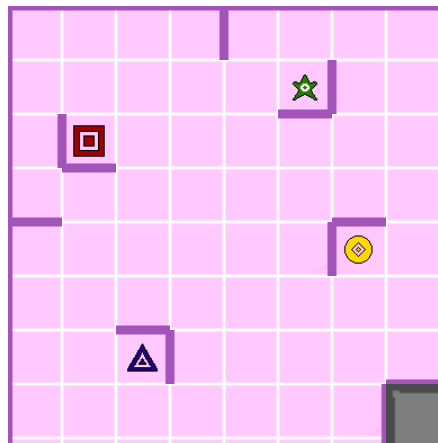
\includegraphics[scale=0.2]{images/bout.png}
                            
                            \vspace{0.5cm}
                            
                            \begin{tikzpicture}
                                \draw (0,0) rectangle (2,2);
                                \draw[dotted] (0,1) -- (2,1);
                                \draw[dotted] (1,0) -- (1,2);
                                \node (4) at (0.5,0.5) {4};
                                \node (3) at (1.5,0.5) {3};
                                \node (2) at (1.5,1.5) {2};
                                \node (1) at (0.5,1.5) {1};
                            \end{tikzpicture}
                        \end{figure}
                      
                        
                        
                
                    \end{column}
                    \begin{column}{6cm}
                        \begin{enumerate}
                            \item Application d'une rotation de 90 degrés du mini-plateau:
                            
                            \begin{figure}
                                \centering
                                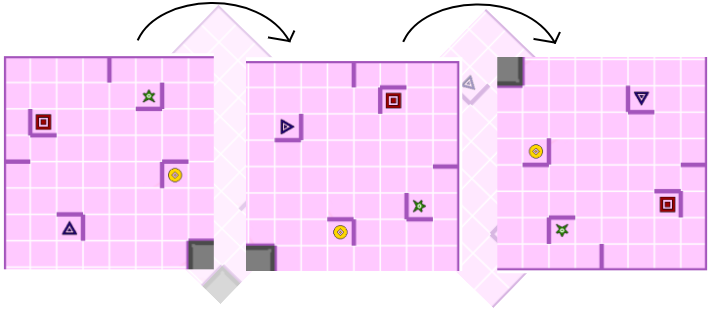
\includegraphics[scale=0.2]{images/rotation.png}
                            \end{figure}
                            
                            \item  Application d'une rotation de 90 degrés de chaque case du mini-plateau:
                              
                             \begin{figure}
                                \centering
                                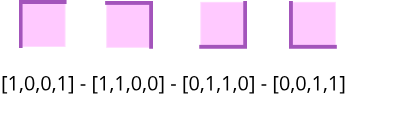
\includegraphics[scale=0.4]{images/rotaCase.png}
                            \end{figure}
                            
                        \end{enumerate}
                    \end{column}
                \end{columns}
                
               
             
            
            \end{frame}
%---------------------------------------------------------------
    \subsection{Déplacements et collisions des robots}
        \begin{frame}{Déplacements et collisions des robots}
            \begin{figure}[H]
                \centering
                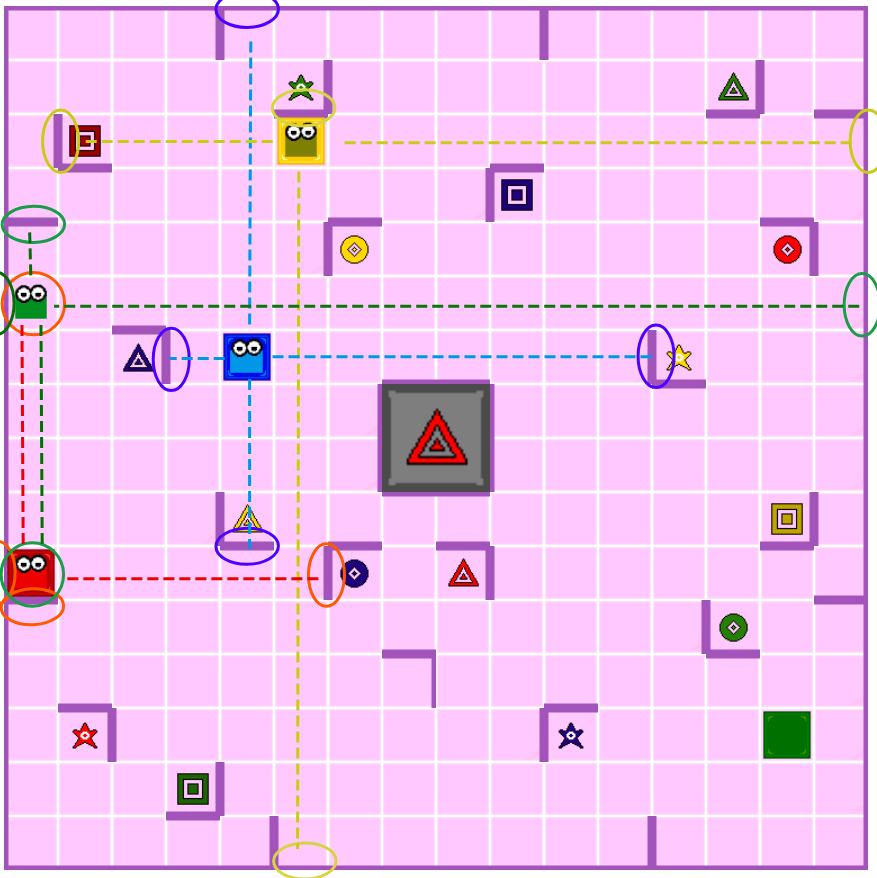
\includegraphics[scale=0.15]{images/collision.png}
            \end{figure}
            
            \begin{figure}[H]
                \centering
                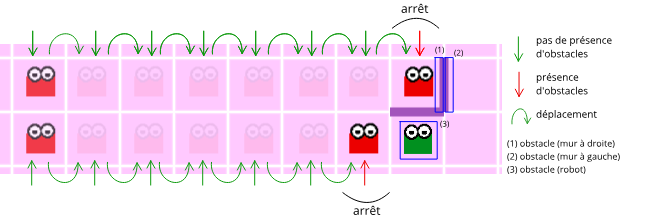
\includegraphics[scale=0.4]{images/deplacements.png}
            \end{figure}
        \end{frame}
%---------------------------------------------------------------
        \begin{frame}{Algorithme de déplacements des robots}
    
            \begin{center}
                \scalebox{0.5}{
                    \begin{algorithm}[H]%-------------------------------------------
                        \DontPrintSemicolon
                        \KwIn{La direction de déplacement}
                		\If{$direction == haut$}{
                			\While{$pas\ de \ mur\ en\ haut\ de\ la\ case\ actuelle$ \textbf{et} $pas\ de\ 
                			mur\ en\ bas\ de\ la\ case\ suivante $ \textbf{et}  $  !estUneCollisionRobot(direction, robot)$}{
                				$deplacement\ d'une\ case\ vers\ le\ haut$
                			}
                		}
                		\uElseIf{$direction == bas$}{
                			
                			\While{$pas\ de \ mur\ en\ bas\ de\ la\ case\ actuelle$ \textbf{et} $pas\ de\ 
                			mur\ en\ haut\ de\ la\ case\ suivante $ \textbf{et}  $  !estUneCollisionRobot(direction, robot)$}{
                				$deplacement\ d'une\ case\ vers\ le\ bas$
                			}
                		}
                		\uElseIf{$direction == gauche$}{
                			\While{$pas\ de \ mur\ a\ gauche\ de\ la\ case\ actuelle$ \textbf{et} $pas\ de\ 
                			mur\ a\ droite\ de\ la\ case\ suivante $ \textbf{et}  $  !estUneCollisionRobot(direction, robot)$}{
                				$deplacement\ d'une\ case\ vers\ la\ gauche$
                			}
                		}
                		\uElseIf{$direction == droite$}{
                			 \While{$pas\ de \ mur\ a\ droite\ de\ la\ case\ actuelle$ \textbf{et} $pas\ de\ 
                			mur\ a\ gauche\ de\ la\ case\ suivante $ \textbf{et}  $  !estUneCollisionRobot(direction, robot)$}{
                				$deplacement\ d'une\ case\ vers\ la\ droite$
                			}
                		}
                        \caption{\sc Déplacement d'un robot jusqu'à collision}
                    \end{algorithm}%-------------------------------------------
                }
            \end{center}
        \end{frame}
%---------------------------------------------------------------
    \subsection{Sélection d'un robot}
        \begin{frame}{Sélection d'un robot}
            \begin{figure}[H]
                \centering
                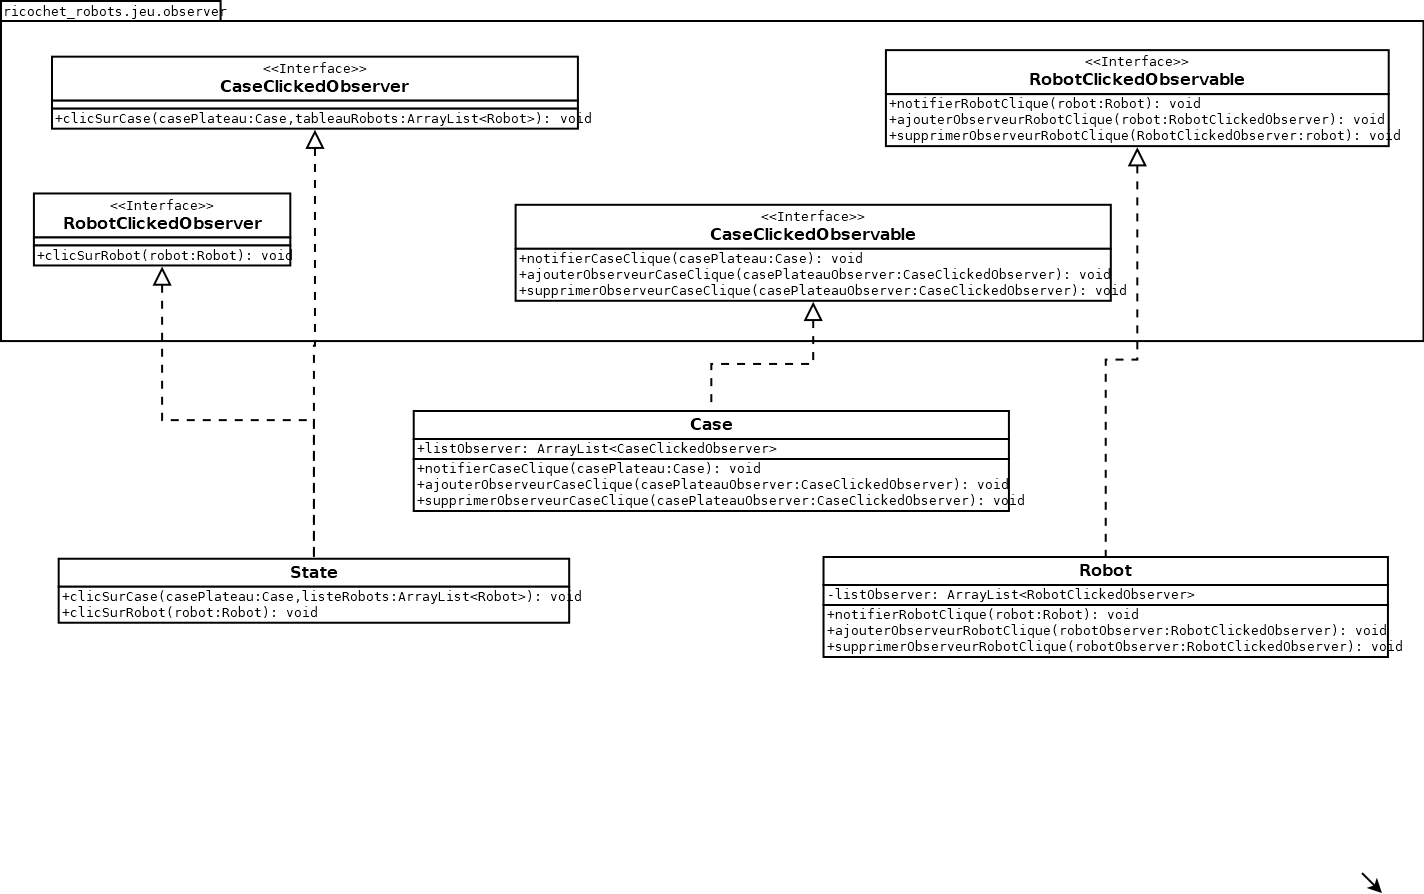
\includegraphics[scale=0.2]{images/patternObserver.png}
            \end{figure}
        \end{frame}
%---------------------------------------------------------------
\section{Algorithme A*}
    \subsection{Première approche : l’algorithme BFS}
        \begin{frame}{Première approche : l’algorithme BFS}
            \begin{itemize}
                \item  Idée: Commencer par implémenter un algorithme de parcours de noeud et de le modifier afin de le transformer en algorithme A*.
                \item Avantage: Permet de bien comprendre le principe de parcours de noeud de ce type d'algorithme.
            \end{itemize}
            
            \vspace{1cm}
           
            L'algorithme BFS (Breadth First Search en anglais), est un algorithme permettant le parcours d'un graphe ou d'un arbre étage par étage.
            
            \vspace{0.5cm}
              
            \scalebox{0.35}{
                    \begin{tikzpicture}[scale=0.75]
                        \node[fill=orange,draw=black,text=black, shape=circle] (S0) at (3,4) {S0};
                        \node[fill=pink,draw=black,text=black, shape=circle] (S1) at (1,2) {S1};
                        \node[fill=pink,draw=black,text=black, shape=circle] (S2) at (5,2) {S2};
                        \node[draw=black,text=black, shape=circle] (S3) at (0,0) {S3};
                        \node[draw=black,text=black, shape=circle] (S4) at (2,0) {S4};
                        \node[draw=black,text=black, shape=circle] (S5) at (4,0) {S5};
                        \node[draw=black,text=black, shape=circle] (S6) at (6,0) {S6};
                        
                        \draw[<-] (S0) -- (S1);
                        \draw[<-] (S1) -- (S3);
                        \draw[<-] (S1) -- (S4);
                        \draw[<-] (S0) -- (S2);
                        \draw[<-] (S2) -- (S5);
                        \draw[<-] (S2) -- (S6);
                    \end{tikzpicture}
                    \begin{tikzpicture}[scale=0.75]
                        \node[fill=green,draw=black,text=black, shape=circle] (S0) at (3,4) {S0};
                        \node[fill=orange,draw=black,text=black, shape=circle] (S1) at (1,2) {S1};
                        \node[fill=pink,draw=black,text=black, shape=circle] (S2) at (5,2) {S2};
                        \node[fill=pink,draw=black,text=black, shape=circle] (S3) at (0,0) {S3};
                        \node[fill=pink,draw=black,text=black, shape=circle] (S4) at (2,0) {S4};
                        \node[draw=black,text=black, shape=circle] (S5) at (4,0) {S5};
                        \node[draw=black,text=black, shape=circle] (S6) at (6,0) {S6};
                        
                        \draw[<-] (S0) -- (S1);
                        \draw[<-] (S1) -- (S3);
                        \draw[<-] (S1) -- (S4);
                        \draw[<-] (S0) -- (S2);
                        \draw[<-] (S2) -- (S5);
                        \draw[<-] (S2) -- (S6);
                     \end{tikzpicture}
                     \begin{tikzpicture}[scale=0.75]
                        \node[fill=green,draw=black,text=black, shape=circle] (S0) at (3,4) {S0};
                        \node[fill=green,draw=black,text=black, shape=circle] (S1) at (1,2) {S1};
                        \node[fill=orange,draw=black,text=black, shape=circle] (S2) at (5,2) {S2};
                        \node[fill=pink,draw=black,text=black, shape=circle] (S3) at (0,0) {S3};
                        \node[fill=pink,draw=black,text=black, shape=circle] (S4) at (2,0) {S4};
                        \node[fill=pink,draw=black,text=black, shape=circle] (S5) at (4,0) {S5};
                        \node[fill=pink,draw=black,text=black, shape=circle] (S6) at (6,0) {S6};
                        
                        \draw[<-] (S0) -- (S1);
                        \draw[<-] (S1) -- (S3);
                        \draw[<-] (S1) -- (S4);
                        \draw[<-] (S0) -- (S2);
                        \draw[<-] (S2) -- (S5);
                        \draw[<-] (S2) -- (S6);
                     \end{tikzpicture}
                     
                     
                    \begin{tikzpicture}[scale=0.75]
                        \node[fill=green,draw=black,text=black, shape=circle] (S0) at (3,4) {S0};
                        \node[fill=green,draw=black,text=black, shape=circle] (S1) at (1,2) {S1};
                        \node[fill=green,draw=black,text=black, shape=circle] (S2) at (5,2) {S2};
                        \node[fill=orange,draw=black,text=black, shape=circle] (S3) at (0,0) {S3};
                        \node[fill=pink,draw=black,text=black, shape=circle] (S4) at (2,0) {S4};
                        \node[fill=pink,draw=black,text=black, shape=circle] (S5) at (4,0) {S5};
                        \node[fill=pink,draw=black,text=black, shape=circle] (S6) at (6,0) {S6};
                        
                        \draw[<-] (S0) -- (S1);
                        \draw[<-] (S1) -- (S3);
                        \draw[<-] (S1) -- (S4);
                        \draw[<-] (S0) -- (S2);
                        \draw[<-] (S2) -- (S5);
                        \draw[<-] (S2) -- (S6);
                    \end{tikzpicture}
                      \hspace{3cm}
                    \begin{tikzpicture}
                        \draw[dotted] (0,0) rectangle (8,3.5);
                        \draw[fill=green] (1,2.75) circle (0.25);
                        \draw[fill=orange] (1,2) circle (0.25);
                        \draw[fill=pink] (1,1.25) circle (0.25);
                        \draw (1,0.5) circle (0.25);
                        
                        
                        \node (dE) at (3,2.75) {noeud exploré};
                        \node (ecE) at (4.35,2) {noeud en cours d'exploration};
                        \node (ecE) at (3.25,1.25) {noeud à explorer};
                        \node (nE) at (3.05,0.5) {noeud inconnu};
                    \end{tikzpicture}
            }
        \end{frame}
%---------------------------------------------------------------
    \subsection{Application au Ricochet Robots}
        \begin{frame}{Application au Ricochet Robots}
            Pour de déplacement d'un seul robot:
            \begin{figure}
                \centering
                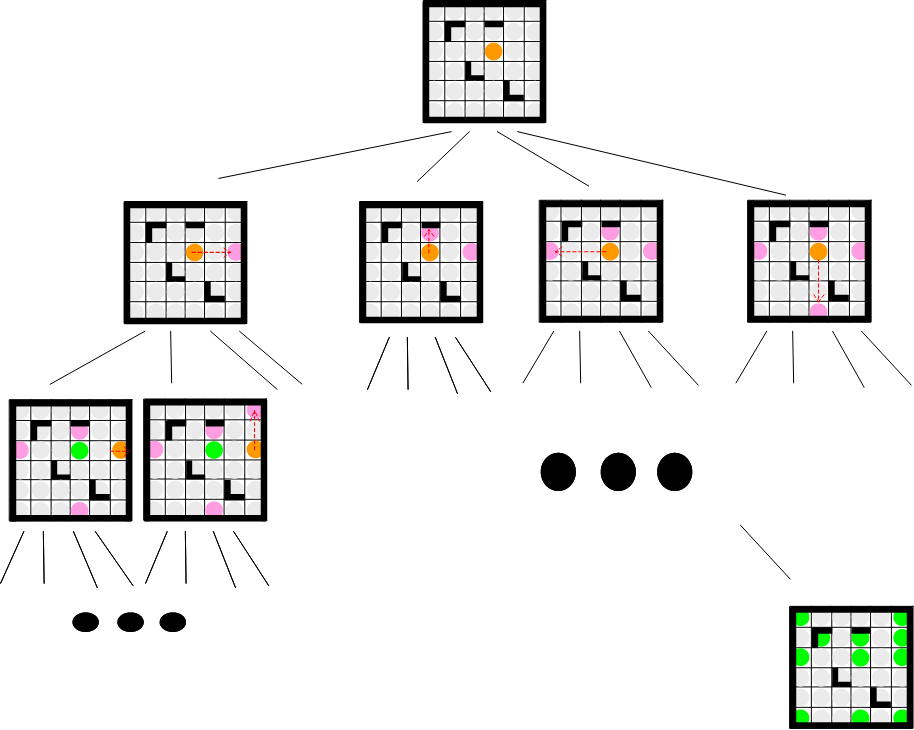
\includegraphics[scale=0.25]{images/bfsRicochet.png}
            \end{figure}
        \end{frame}
%---------------------------------------------------------------
        \begin{frame}{Comparaison entre les algorithmes BFS et A*}
            
                Similarités:
                \begin{itemize}
                    \item Algorithmes de parcours de noeuds, permettent la recherche de chemin.
                    \item Le noeud suivant qui est pris correspond au premier élément d'une liste de noeuds à explorer.
                \end{itemize}
                
                Problèmes au BFS:
                \begin{itemize}
                    \item La liste de noeuds à explorer contient suite à suite les voisins du noeud courant.
                    \item Parcours long en testant tout les cas possibles.
                    \item Parcours de noeuds inintéressant à la résolution du problème.
                \end{itemize}
                
                Solution:
                \begin{itemize}
                    \item Prioriser certains coups afin atteindre plus rapidement le noeud solution.
                \end{itemize}
        \end{frame}
%---------------------------------------------------------------
    \subsection{Optimisation de l'A*}
        \begin{frame}{Pourquoi une heuristique?}
            \begin{itemize}
                \item Permet d'aller plus rapidement vers la solution.
                \item  Type d'heuristique le plus connu: heuristique du vol d'oiseau.
                
                \begin{itemize}
                    \item Calcule la distance du pion actuel par rapport à l'objectif
                    \item Priorise les états qui se rapprochent de l'objectif
                \end{itemize}
            \end{itemize}
%---------------------------------------------------------------
            \begin{figure}
                \centering
                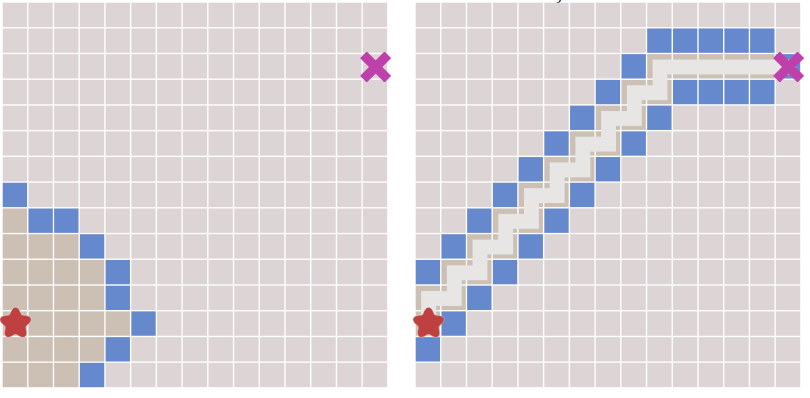
\includegraphics[scale=0.35]{images/2.PNG}
                \caption{Algorithme A* avec et sans heuristique après 23 coups\cite{redblob}}
            \end{figure}
            Cependant, cette heuristique n'est pas adaptée au Ricochet Robots.
        \end{frame}
%---------------------------------------------------------------
    \begin{frame}{Mise en place de l'heuristique}
         \begin{figure}
            \centering
            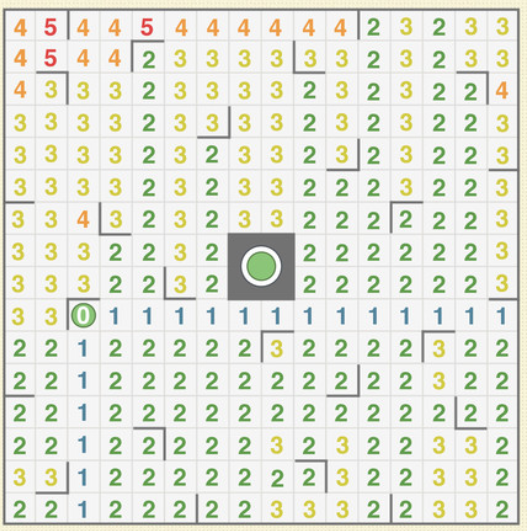
\includegraphics[scale=0.5]{images/mapHeuristique.PNG}
            \caption{Exemple de carte heuristique pour le Ricochet Robots\cite{heurist}}
        \end{figure}
    \end{frame}
%---------------------------------------------------------------
    \subsection{Application de l'algorithme A*}
        \begin{frame}{Application de l'algorithme A*}
            \scalebox{0.4}{
             \begin{algorithm}[H]%-------------------------------------------
                
                \DontPrintSemicolon
                \KwIn{L'etat initial}
                $etatInitial \gets l'etat\ initial$;
                
                $PriorityQueue<State> frontier \gets new\ PriorityQueue<>()$;
                
            	$HashMap<State,State> cameFrom \gets new\ HashMap<>()$;
            	
            	$HashMap<State,Integer> costSoFar \gets new\ HashMap<>()$;
            	
            	$ArrayList<State> path \gets new\ ArrayList<>()$;
            	
            	$ArrayList<Robot> listRobot \gets new\ ArrayList<>()$;
            	
            	$ArrayList<Deplacement> listDeplacement \gets new\ ArrayList<>()$;
    
    	        $etatInitial.setValCost(0)$;
    	        
    	        $frontier.add(etatInitial)$;
    	        
    	        $cameFrom.put(etatInitial, null)$;
    	        $costSoFar.put(etatInitial, cout\ de\ l'etat\ initial)$;
        
            	\While{$frontier\ n'est\ pas\ vide$}{
    		
    		        $noeudEnCours \gets frontier.poll()$;
    		
            		\If{$objectif\ atteint$}{
            			$etatFinal \gets noeudEnCours$;
            			
            			$break$;
            		}
            		
            		\For{$chaque\ direction$}{
            			\For{$chaque\ robot$}{
            				$etatSuivant \gets noeudEnCours.etatSuivant(direction, robot)$;
            				
                            $newCost \gets cout\ de\ l'etat\ suivant\ + 1 + heuristique\ de\ l'etat\ suivant$;
            
            				\If{$l'etat\ suivant\ est\ nouveau$ \textsc{or} $le\ cout\ de\ l'etat\ suivant\ est\ plus\ petit\ que\ celui\ de la liste$}{
            					$costSoFar.put(etatSuivant, newCost)$;
            					$etatSuivant \gets cout\ de\ l'etat\ suivant\ + 1$;
            					$frontier.add(etatSuivant)$;
            					$cameFrom.put(etatSuivant, noeudEnCours)$;
            				}
            			}
            		}
            	}
        	    \caption{\sc Algorithme A*}
            \end{algorithm}
                
                
            \begin{algorithm}[H] 
    	        $current \gets etatFinal$;
    
            	\While{$current != etatInitial$ {and} $ current != null$}{
            		$path.add(current)$;
            		
            		$current = cameFrom.get(current)$;
            	}
            	\If{$l'etat\ actuel\ existe$}{
            		$path.add(etatInitial)$;
            
            		\For{$chaque\ etat\ du\ chemin$}{
            			$listDeplacement.add(dernier\ deplacement\ de\ l'etat)$;
            			
            			$listRobot.add(dernier\ deplacement\ de\ robot\ de\ l'etat)$;
            		}
            
            		$reverse(listRobot)$;
            		$reverse(listDeplacement)$;
            
            		\For{$chaque deplacement de robot$}{
            			affiche le robot et la direction à effectuer
            		}
            	}
            	\Else{
            		affiche "pas de solution"
            	}
                
            \end{algorithm}%-------------------------------------------
            }
        \end{frame}
%---------------------------------------------------------------
    \section{Démonstration}
        \begin{frame}{Démonstration de l'application}
            Nous allons procéder à la démonstration de l'application du Ricochet Robots.
        \end{frame}
%---------------------------------------------------------------
    \section{Conclusion}
        \begin{frame}{Conclusion}
            Ce projet était très intéressant. Nous ne connaissions pas le Ricochet Robots et c'était intéressant de se pencher sur les règles de ce jeu et de le recréer afin de pouvoir y jouer autrement que sous forme physique.
    
            \vspace{0.5cm}
            Améliorations possibles:
            \begin{itemize}
                \item La mise en place du jeton spirale. 
                \item La mise en place d'un système de score.
                \item Une mise en duel entre l'IA et le joueur.
                \item L'ajout ou la suppression de robots sur le plateau.
                \item L'ajout d'obstacles (et/ou de malus) ou de bonus sur le plateau. 
                \item Mise en place d'un système de difficulté.
                \item Mise en place du délai pour la réflexion et pour la réalisation des mouvements.
            \end{itemize}
        \end{frame}
%---------------------------------------------------------------
\begin{frame}{Bibliographie}
    Références:
    \bibliographystyle{unsrt}
    \bibliography{bibliography}
\end{frame}
%---------------------------------------------------------------
\end{document}